
\documentclass[12pt]{article}
%\setlength{\oddsidemargin}{0in}
%\setlength{\evensidemargin}{0in}
%\setlength{\textwidth}{6.5in}
%\setlength{\parindent}{0in}
%\setlength{\parskip}{\baselineskip}
\thispagestyle{empty}
\usepackage{fullpage}
\usepackage{amsmath,amsthm,amsfonts}
\usepackage{graphicx, graphics}
\usepackage[usenames,dvipsnames]{color}

\definecolor{darkyellow}{rgb}{.929412,.8314,0}
\definecolor{brightgreen}{rgb}{.439,.824,.0863}


\newtheorem*{thm}{Theorem}

\begin{document}

%=======================================================
\begin{center}
{\bf ``The most jaw-droppingly pompous soliloquy ever delivered in a mainstream Hollywood movie [BBC Review]:"}
\end{center}

Good morning. In less than an hour, aircraft from here will join others from around the world. And you will be launching the largest aerial battle in the history of mankind. ``Mankind." That word should have new meaning for all of us today. We can't be consumed by our petty differences anymore. We will be united in our common interests. Perhaps it's fate that today is the Fourth of July, and you will once again be fighting for our freedom... Not from tyranny, oppression, or persecution... but from annihilation. We are fighting for our right to live. To exist. And should we win the day, the Fourth of July will no longer be known as an American holiday, but as the day the world declared in one voice: ``We will not go quietly into the night!" We will not vanish without a fight! We're going to live on! We're going to survive! Today we celebrate our Independence Day!\\

-President Thomas Whitmore

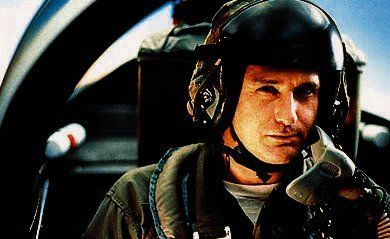
\includegraphics[scale=0.25]{bps.jpg}


\end{document}
